%%% Preâmbulo: define o tipo de documento, linguagens utilizadas, pacotes e as características da capa.

% Tipo de Documento
\documentclass[12pt, a4paper]{article} 

% Formato do documento e pacotes importantes
\usepackage[utf8]{inputenc} % codificação de strings
\usepackage[lmargin=3cm,tmargin=3cm,rmargin=2cm,bmargin=2cm]{geometry} % bordas ABNT
\usepackage[onehalfspacing]{setspace} % espaçamento 1.5cm
\usepackage[T1]{fontenc}
\usepackage[brazil]{babel}
\usepackage{graphicx, xcolor, comment, enumerate, multirow, multicol, indentfirst, hyperref} % Pacotes Essenciais
\usepackage{amsmath, amsthm, amsfonts, amssymb, dsfont, mathtools, blindtext} % Pacotes de Matemática

% Cabeçalho
\title{Resumo de LaTeX}
\author{Bruno Marcelino}
\date{\today}

%%% Corpo do Documento: escreve o texto
\begin{document}

\maketitle % Importa o cabeçalho para o documento nesse local

% Resumo

\begin{abstract}
    Este é um resumo de como utilizar algumas ferramentas do LaTeX.
\end{abstract}

% Sumário 

\tableofcontents

% Seções
\section*{Introdução}

    A ferramenta LaTeX permite criar longos documentos padronizados, com um rígido controle de formatação. O objetivo primário é a redação do documento, para assim logo depois realizar o processo da formatação de uma forma sistematizada.
    
    Podem ser realizadas citações, referências bibliográficas, divisão do texto em tópicos, organização das figuras, entre outros.

\subsection{Preâmbulo}

    Define o tipo de documento, linguagens utilizadas, pacotes e as características da capa.
    
\subsection{Environment}
    
    Iniciam partes do documento que devem ser formatadas de forma diferente. Utilizamos a palavra-chave \textbf{begin} para abrir um environment.

\section{Texto}

\subsection{Destaque de Texto}
Lorem Ipsum is simply \textbf{dummy} (Negrito)
text of the printing \textit{and} (Itálico)
typesetting industry. \underline{Lorem} (Sublinhado)
Ipsum has been the industry's.

\subsection{Lista de Itens}
\subsubsection{Lista não Ordenada}
\begin{itemize}
    \item $P_{0}$ é o valor da ação no presente;
    \item $D_{0}$ é o dividendo presente;
    \item $g$ é a taxa de crescimento dos dividendos;
    \item $r$ é a taxa de desconto.
\end{itemize}
\subsubsection{Lista Ordenada}

\begin{enumerate}
    \item $P_{0}$ é o valor da ação no presente;
    \item $D_{0}$ é o dividendo presente;
    \item $g$ é a taxa de crescimento dos dividendos;
    \item $r$ é a taxa de desconto.
\end{enumerate}

\subsection{Hyperlink}
\href{https://www.cfainstitute.org/-/media/documents/book/rf-lit-review/2012/rflr-v7-n1-1-pdf.ashx}{Podemos inserir links em pedaços de texto.}

\section{Imagens}
    As imagens devem ser importadas em conjunto com a biblioteca \textit{graphicx}.

\graphicspath{ {images/} } % Caminho relativo da pasta (no projeto do overleaf) onde estão os gráficos

\begin{figure}[h]
    \centering
    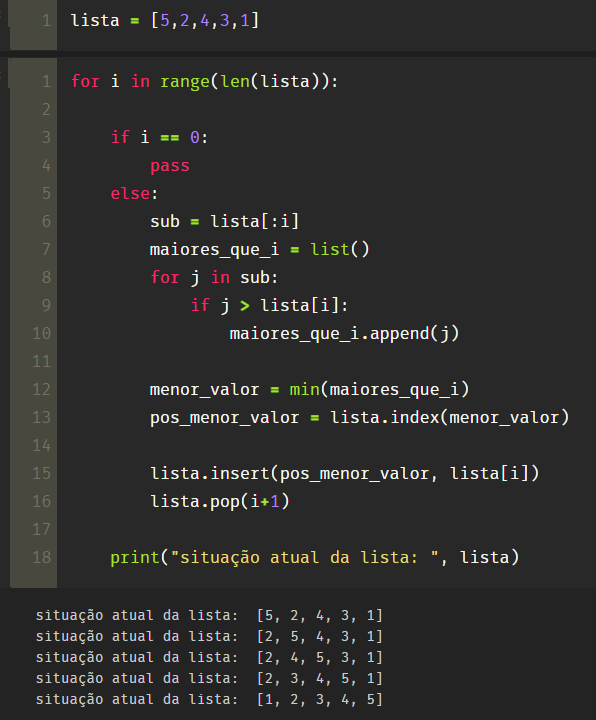
\includegraphics[scale = 0.35, width = 0.25\textwidth]{Screenshot_22} % sem espaços em branco ou muitos pontos
    \caption{Imagem Aleatória}
    \label{script} % declara a figura como uma variável
\end{figure}

\section{Tabelas}

\begin{center}
    \begin{table}[h!]
        \begin{tabular}{||c|c|c||} % número de colunas, todas centralizadas (opções: r, c e l) e com bordas (||, {} e [])
         \hline
         cell1 & cell2 & cell3 \\ % pula linha
         \hline
         cell4 & cell5 & cell6 \\ % pula linha
         \hline
         cell7 & cell8 & cell9
         \hline
        \end{tabular}
    \caption{Tabela aleatória}
    \label{Tabela}
    \end{table}[h!]
\end{center}

\section{Matemática}

\subsection{Equações}
Devemos baixar o pacote \textit{amsmath}.

\subsubsection{Modo Inline}

A equação $e = mc^2$ pode ser escrita na linha de texto.

\subsubsection{Modo Display Sem Enumeração}
$P_{0}=\frac{D_{0}(1+g)}{r-g}$

\subsubsection{Modo Display Enumerado}
\begin{equation}
    PV=\left[\frac{C_{1}}{(1+r)^{1}}+\frac{C_{2}}{(1+r)^{2}}+\frac{C_{3}}{(1+r)^{3}} \ldots+\frac{C_{n}}{(1+r)^{n}}\right] = \sum^n_{i = 1} \frac{CF_{i}}{(1+r)^i}
\end{equation}

\subsubsection{Exemplo Completo}

Subscripts in math mode are written as $a_b$ and superscripts are written as $a^b$. These can be combined an nested to write expressions such as

\[ T^{i_1 i_2 \dots i_p}_{j_1 j_2 \dots j_q} = T(x^{i_1},\dots,x^{i_p},e_{j_1},\dots,e_{j_q}) \]
 
We write integrals using $\int$ and fractions using $\frac{a}{b}$. Limits are placed on integrals using superscripts and subscripts:

\[ \int_0^1 \frac{dx}{e^x} =  \frac{e-1}{e} \]

Lower case Greek letters are written as $\omega$ $\delta$ etc. while upper case Greek letters are written as $\Omega$ $\Delta$.

Mathematical operators are prefixed with a backslash as $\sin(\beta)$, $\cos(\alpha)$, $\log(x)$ etc.

\subsection{Matrizes}
$
    \left[ % tipo de contorno 
    \begin{array}{ccc}
    3 & 2 & 3 \\
    2 & 1 & 2 \\
    1 & 1 & 1 
    \end{array}
    \right] % tipo de contorno 
$

\end{document}
